\documentclass{article}

\usepackage{authblk} % author details and affiliations
\usepackage{multicol} % two column arrangement
\usepackage{natbib} % parenthetical apa citation
\usepackage{float} % hard format figures
\usepackage{abstract} % writing abstract
\usepackage{chemformula} % write chemical formulae
\usepackage{ragged2e} % align document
\usepackage[utf8]{inputenc} % to accomodated for utf-8 encodings
\usepackage[a4paper,left=2cm,right=2cm,top=2.5cm,bottom=2.5cm]{geometry} % adjust margins
\usepackage{amsmath} % align math equations and their descriptions
\usepackage{array} % used to perform column width sizing along with centering
\usepackage[center]{caption} % center figure and table captions
\usepackage{subcaption} % for using the subfigure environment
\usepackage{gensymb} % generate symbols. used for the degree symbol
\usepackage{hyperref} % referencing with backlinks and name of reference type.


\newcolumntype{x}[1]{>{\centering\arraybackslash\hspace{0pt}}p{#1}} % new columns with type

\graphicspath{ {./images/} } % path to image files

\title{\line(1, 0){500}\\\vskip 0.5em
Analysis Of The Morphological And Mechanical Characterization Of Aluminium Matrix Composite Reinforced With Chitosan\\
\line(1, 0){500}}

\author[1]{Victor Ezekiel \thanks{victor.ezekiel@stu.cu.edu.ng}}
\author[1]{Udoye Nduka \thanks{Corresponding Author: nduka.udoye@covenantuniversity.edu.ng}}
\affil[1]{Department of Mechanical Engineering, Covenant University}
\date{\today}


\begin{document}
    \let\ref\autoref % uses the autoref command for \ref

    \maketitle % display image

    \begin{abstract}
        
        \noindent
        Aluminium is quintessential metal to human civilization. As noted in literature, reinforcements provide material property customization targeted at specific engineering needs. Recent studies acknowledge that convectional ceramic particulate could be replaced by several agricultural in the development of aluminium matrix composites because of selected for their low cost and relative ubiquity. This study explores development of aluminium matrix composite from AA6061 alloy reinforced with chitosan particulates at weight proportions (3, 6, 9, and 12wt.\%). The study further characterizes the developed composites using Scanning Electron Microscopy (SEM), Energy Dispersive Spectroscopy (EDS), X-ray Diffractometer (XRD), hardness, tensile and thermal and electrical conductivity test techniques. Results indicated that increasing chitosan content up to 10 wt. \% enhanced the hardness performance, while tensile strength of the composites increased sporadically, as SEM images observed reinforcement links embedded in grain boundaries. However, the thermal and electrical conductivity diminished due to the addition of chitosan particulates to the alloy matrix. The overall study showed great potential  of chitosan polymer as reinforcement to aluminium alloy.
    \end{abstract}

    \begin{multicols}{2}
        \section{\raggedright Introduction}
            \justify
            The evolution of the engineering discipline has intimated developments of advanced materials to sustain equipment performance in austere conditions confronted in the energy, aerospace, automotive and construction industries. Scientists have purported metal matrix composites MMC for the enhancement of material strength to weight ratio, dilapidation resistance, and conductivity in industrial machinery \citep{Mansoor2016Carbon,Orhadahwe2020review,Pawar2018Comprehensive}. Aluminium, a copious lightweight metal, has been extensively applied in the fabrication of automobiles and aeroplanes parts, components, and structures. Yet, the laudable corrosion resistance, substantial thermal and electrical conductivity of aluminium influence its utilization as base material in household utensils, sporting equipment, appliances, and electronic devices. Thus, extensive research has sought to extend the application of aluminium by improving certain desirable properties. Subsequently, scientist have developed and investigated aluminium matrix composite reinforced with ceramics: \ch{Al2O3} , aluminium oxide; SiC, silicon carbide \ch{SiO2}, silicon oxide; \ch{B4C}, boron carbide; and \ch{TiC}, titanium carbide. However, the prevalent interest on sustainability and the impact of human activities to the environment highlight pollution produced from the synthesis of ceramic reinforcements.  Furthermore, concerns over the availability and cost of aluminium metal matrix composites (AMMCs) reinforced with ceramic composites have limited AMMC adoption at a large scale.

            Accordingly, cost efficient synthesis technique, most notably stir casting, have been adopted as well as the utilization of agricultural waste material as reinforcement in AMMCs. Therefore, agro–waste like rice husk, breadfruit seed, bagasse seed, eggshell, coconut husk, and aloe vera have gained prominence in industry as preferred alternatives to ceramic reinforcements, moreover numerous research work is dedicated to exploring reinforcement materials to attain superior corrosion, mechanical and morphological properties to that of unreinforced aluminium. These waste derivatives of terrestrial and aquatic animals as well as plants have been found to attenuate environmental impact and improve material performance. Hence, this research seeks to employ chitosan particulates of 90 microns sieve size as reinforcement to the AA6061 aluminium alloy matrix developed via stir casting and characterize the composites mechanical, morphological, thermal, and electrical properties.
        \section{\raggedright Literature review}
            \subsection{\raggedright Ceramic reinforcements of aluminium alloys}
                Reinforcement of metals to achieve superior performance predates modern civilization \citep{Chawla2012Composite,Tsangarakis1987}
                , however preliminarily contemporary applications of aluminium composites were in the development of aircrafts \citep{LinoAlves2016Metal}. Driven, Over the years, scientists have explored reinforcement materials particularly ceramic particulates in developing AMMCs. The ceramic particulate, alumina, \ch{Al2O3}, is highly prioritized in reinforcements selection for aluminium and its alloys, which is attributed to empirically proven superiority in hardness, tensile and stiffness properties of aluminium matrix composites composite \ch{Al2O3} \citep{Bansal2013Experimental}. The analysed impact resistance of squeeze cast alumina reinforced AC-44200 further emphasizes the advantage of reinforcing aluminium alloy in alumina, when \cite{Kurzawa2018Analysis} appraised ballistic resistance of the unreinforced alloy and the developed composite. The authors discovered that the aluminium alloy with 20 and 40 per cent alumina by volume effectively dissipated 30 \% and 50 \% impact energy causing a significant retardation in projectile velocity. This interesting discovery proved relevant as ballistic shield would experience a significant reduction in weight to effectiveness in military armours. Subsequently, an investigation of the mechanical and morphological effects of AA6061 reinforcement with hybrid particulates consisting of boron nitride and alumina. \cite{Gopinath2020Enhancing} demonstrated an improvement in mechanical strength of the alloy. Increasing BN proportions in the composites led to significant improvements in compressive, impact, hardness, and tensile strengths. The authors further noted enhanced dilapidation resistance of wear and corrosive conditions in developed composite.

                Likewise, ceramics like silicon carbide have been explored by researchers as reinforcements for aluminium, metal or alloy, matrix. Heat dissipation performance being critical in aircrafts and automobiles, \cite{Manivannan2017Thermal} examined the as cylindrical fins for various ceramic fillers, of AA 6061 matrix. The authors found most significant improvement in thermal dissipation properties, conductivity and heat transfer coefficient correspondingly greater in composites reinforced with boron nitride, alumina, and silicon carbide over the as-cast AA 6061 alloy. Such Improvements are largely attributed to quantities of newly formed phases like \ch{Fe2SiAl8} and \ch{Al15(Fe,Mn)3Si} dispersed within the previous vastly mono-atomic matrix \citep{Mandal2013Effect}. However, \cite{Carron2008Thermal} noted that with increased presence of diamond in the hybrid reinforcements, silicon carbide + diamond, thermal and electrical conductivity of the aluminium composite. confirmed this to be the detrimental effect of Silicon precipitate phases in the composite and prolonged contact of silicon and molten aluminium matrix as observed in composite manufactured with pressure infiltration fabrication technique. Thus, the introduced diamond ensured less silicon availability for dissolution.

                Furthermore, titanium carbide reinforcements of AA 6061 in in-situ reaction with both silicon carbide and \ch{k2TiF6} expressed with evenly dispersed TiC particulates and precipitated intermetallic phases over the standard alloy were formed in \citep{LIJAY2016Microstructure}. The authors further noted an almost linear improvement in hardness, UTS and percentage elongation with increasing \ch{TiC} presence. More recently, \cite{Kumar2018Experimental} found graphite–titanium carbide hybrid reinforcement of aluminium in varying weight proportions showed enhanced wear resistance over unreinforced alloy. The 4 wt. \% \ch{TiC} sample exhibited highest hardness and tensile strength gains over AA 7075. Finally, \cite{Bandhu2018Characterization}examined behaviours of various ceramic particulate reinforcements in AA 7075. They studied reinforcing addition of 15 wt. \% of \ch{Al2O3}, \ch{SiC}, \ch{B4C} and \ch{TiB2}. The authors discovered maximum improvements in hardness, tensile, impact strength performance of composites over as-cast alloy in the \ch{B4C} reinforced sample. Thus, they endorsed the selection of \ch{B4C} particulates for customized aluminium alloy improvements in mechanical behaviour.

            \subsection{\raggedright Agricultural waste reinforcements of aluminium}
                Recently, the metallurgy research has focused on reinforcements of aluminium matrix composite with agricultural waste materials. While being economical, these waste materials undergo value recycle satisfying the modern concerns on sustainability and ecological impact of manufacturing activities. However, extensive investigations are conducted to compare performance gains of these composites and properties of unreinforced aluminium alloys as well as AMMCs reinforced with conventional materials (i.e., ceramics).
                \subsubsection{\raggedright Wood}
                    Significant quantities of wood have been used throughout civilization in construction of roads, bridges, and buildings \citep{Owoyemi2016Sustainable}. However, one of man’s most renewable, now facing shortage have inspired researchers and environmentalists to continually explored sustainable application of the organic fibre in engineering materials such as aluminium composites \citep{Gallo2013Tailoring,Lu2015Reinforced}. The results of these research bring ecological preservation worldwide and economic gains to developing cities and countries with substantial housing problems. The synthesis of waste wood particulate reinforced aluminium reinforced in \cite{Omoniyi2021Mechanical} experienced decreased density with addition of reinforcements. The authors also noted that 97.69 MPa ultimate tensile in 20 wt. \% wood reinforced aluminium matrix composite and 89.4 \% greater impact strength values in 10 \% wood reinforce aluminium composite compared to unreinforced aluminium alloy derived from crushed cans.

                \subsubsection{\raggedright Egg shells}
                    Presently, numerous tons of eggshells are included as calcium supplement in livestock feed \citep{Faridi2018Application}. Furthermore, Egg shells are currently utilized in absorbent of heavy metal in industrial wastewater through climate action programs \citep{Angelis2017Recycling}. The relative ubiquity of poultry industries world-wide justify the exploration of eggshells as potential reinforcement material \citep{Olusesi2021Development}. More so, \cite{Hassan2015Effects} examination of the effects of uniformly dispersed carbonized and uncarbonized eggshell reinforcement in Al-Cu-Mg show increase tensile strength and hardness of the alloy attributed to improved dislocation density caused by the hard eggshell phase. Furthermore, \cite{Dwivedi2016Synthesis} appraised mechanical properties of chicken eggshell particulates in AA 2014. The resulting composite showed enhanced fatigue and tensile strengths, while maintaining low porosity and uniform dispersion of particulates in the alloy matrix. Thus, researchers in \cite{Kumar2020Synthesis} combined ball-milled eggshells and alumina in hybrid reinforcements of heat treated aluminium hybrid composite. The resulting composite provided significantly impressive harness and tensile strength performances over aluminium-egg shells and aluminium-alumina composites. Also, improvements in corrosion resistance transpired with addition of alumina-eggshell reinforcement.

                \subsubsection{\raggedright Coconut husk ash}
                    \textit{Cocos Nucifera} (Coconut) fruit consists of the liquid endocarp, solid endocarp, mesocarp and exocarp \citep{Hutten2007Raw}. The liquid endocarp, coconut milk, is consumed or processed industrially into beverages, while the endocarp is processed into creams and pharmaceuticals \citep{Satheeshan2020Development}. However, the mesocarp, shell, of coconut is generally incinerated or disposed of as waste. With rising oil and gas prices, developing countries synthesize coconut shell into biofuel mixtures to meet energy needs \citep{Husin2018Coconut}. Crop cultivators use CSA stabilize poor laterite soil as well as fertilizer additive \citep{Bonneau2010Coconut,Olusesi2021Development}. Similarly, wastewater treatment systems can apply activate carbon-based absorbent produced from coconut husk for the removal of dyes \citep{Khuluk2019Removal}. Recently, the ash of coconut husk has been identified to contain up to 90\% silica, thus green silica synthesis techniques have been developed to attenuate the adverse ecological impact of industrial synthesis of silica by series of heat and acid treatment of coconut husk \citep{Anuar2020physical}. Therefore, the ash has undergone studies as a secondary reinforcement in AMMCs and an alternative to ceramics for composite development.

                    \cite{Butola2019Effect} reinforced AA6061 with coconut shell ash - SiC mixture using stir casting process in an effort to complement synthetic convention reinforcement, carbide particulates, with agricultural waste coconut shell in composite formation. The developed composite showed improved hardness in Vickers hardness tester over the as-cast alloy. Also, the coconut shell composite expressed higher \% elongation, yield strength and tensile strength  properties that the base alloy. \cite{Subramaniam2018Investigation} investigated the effects of B4C and coconut husk ash reinforcement on mechanical characteristics aluminium 7075. Results show that increasing B4C – CSFA particulate in the alloy increased hardness and enhanced the tensile strength with an observed maximum at 12 wt. \% B4C – CSFA reinforcement. \cite{Raju2017Assessments} identified enhanced Grey-Fuzzy reasoning grade wear performance on aluminium composite with increasing volume of coconut shell ash fabricate via compo-casting technique.

                \subsubsection{\raggedright Rice husk ash}
                    Rice husk (RH) is a silica-rich outer membrane of the rice crop \cite{Hossain2018Rice}. The crop widely grown around the word in paddies is a major agricultural product. The husk a by-product of milled rice crop is traditionally used as a fuel and in cement production. Because the ash contains 90 \% amorphous silica content \cite{Singh2018Rice,Tiwari2017Effect}, numerous industrial application employ it as direct silica alternatives. Silicon oxide and Silicon carbide are themselves good ceramic reinforcements for AMCs. Thus, rice husk ash is a common agricultural waste reinforcement material. For example, \cite{Gladston2017Dry} compo-casted aluminium matrix composites using rice husk ash of varying weight proportions as reinforcement. The authors found that increasing proportions of RHA yielded higher hardness and wear resistance properties of the composite. 

                    Thus, mixture with NaOH, heating, dilution of mixture with DI water, titration and gelatinating; a significant portion of Taungchi RHA silica extraction method \citep{Song2018Surfactant-free}. A unique benefit economically to industry seeking to increase production output of high performing AMCs at a reduced cost. Although, acid or alkaline treatment of RHA increasing silica purity of the product \cite{Hossain2018Rice}, unprocessed ash a product of combustion in a boiler would have served as an energy source and contain as much as 95 \% silica. Also, \cite{Thiagarajan2020Advanced} evaluated using XRD, the crystallinity of pyretic RHA (at up to 1000\degree C) to be 88.6 \%.

                    Further studies on RHA as reinforcement show up to 12 \% increase in ultimate tensile strength of AlSi10Mg \citep{Saravanan2013Effect}. In the investigation on mechanical, morphological and tripological properties of AlSi10Mg reinforced with RHA fabricated via powder metallurgy, \cite{Shaikh_2019} discovered that the maximum hardenss of the composite at 10 wt. \% RHA reinforement was over 15 \% greater that that of unreinforced aluminium. In additon, the authors observed a reduced wear loss using pin-on-disc apparatus on the 5, 10, and 15 wt. \% RHA reinforced samples. The Signal to Noise ratio, larger is better, statistically evaluation of AA6063/10 wt. \% weldements fabricated through sitr casting route show sound weldment  response to varying  welding speed, current and gas flow rate parameter \citep{Saini2020Some}. The varying parameters yeilded consistently inceasing tensile and impact strengths of weldments. Thus, the authors suggested aerospace application of the composite due to its lower density, good weldability and joint strength for fabrication using TIG welding process. Similarly, Friction stir casting of AA6061/RHA provided even dispersion within the alloy matrix observed through FESEM and strong interfacial bonding between RHA particles and the aluminium alloy resulting in enhanced tensile strength of the alloy \citep{Dinaharan2017Influence}. It can be concluded that rice husk ash performance, ubiquity, and low cost of the ash being a waste material evidently cements as a viable alternative to \ch{SiC} and \ch{SiO2} in composite development. 
        \section{\raggedright Experimentation}
            \subsection{\raggedright Material}
                The materials selected for this research are AA6061 and Chitosan particles of sieve size 90$\mu$m.
            \subsection{\raggedright Preparation of Aluminium Matrix composite}
                In this study, stir casting is employed for development of the composites. Stir casting involves the use of a mechanical stirrer to consolidate reinforcement particulates in a molten metal by creating forced vortexes. The process ensures homogeneous distribution of the particulates in the base matrix. Thus, obtained chitosan particles were sun-dried and milled to smooth powder. The particles are then sintered at . 
                % \ref{figure_3_1}
                shows the chitosan particles. AA6061 was heated liquefaction at and place in crucible. At an operating speed of , a mixture of molten AA6061 and sintered chitosan powder are to and stirred vigorously. The mixture is transferred into pre-heated dies and allowed to solidify at room temperature to reveal the AA6061\/chitosan castings. \ref{fig:figure_3_2} shows images of developed aluminium matrix composites.
                \begin{figure}[H]
                    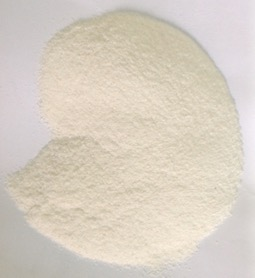
\includegraphics[width = \linewidth]{figure_3_1}
                    \caption{\label{fig:figure_3_1} Dried Chitosan Poweder}
                \end{figure}
                \begin{figure}[H]
                    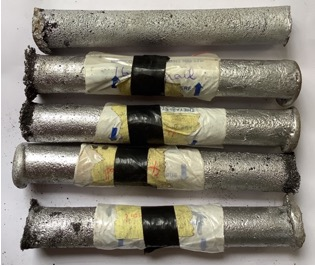
\includegraphics[width = \linewidth]{figure_3_2}
                    \caption{\label{fig:figure_3_2} Cast aluminium matrix composites}
                \end{figure}
        
            \subsection{\raggedright X-ray diffraction analysis}
                X-ray diffraction analysis provides the qualitative crystallographic of the developed samples. Thus, the various composing lattice-structured compounds are identified. XRD technique involves the use of monochromatic collimated X-ray beam incident on sample resulting in scattering of X-rays on interaction with atoms and molecules of the material. These scattered X-rays are diffracted at disparate angles are effects of constructive interference between constituting particles of sample and the incident rays. Characterization of composing phases is obtained by analysis of the various diffraction angles using Bragg’s law given in \ref{eq:equation_1}.
                Moving detector and goniometer pair are used to identify x-rays and measure diffraction angles respectively. The counter is used to record the count-rate of the observed radiation.
                \begin{align}
                    {n\lambda} = {2{D}\sin(\theta)}\label{eq:equation_1}
                \end{align}
                where,\\
                ${d}$ is the wavelength\\
                $\lambda$ is the wavelength\\
                ${n}$ is the order of the diffraction\\
                $\theta$ is the angle of diffraction in degrees\\
            
            \subsection{\raggedright Micro-harness tester}
                The developed composites were subjected to the Brinell hardness test to obtained. The tester provides precise hardness values using Brinell’s technique that accommodates for uneven surfaces better that other test. The samples were tested with a load of 300 Kgf applied to a 10 mm ball indenter at a mass of 100 g for over 15 seconds. Resulting indentations are observed and measured using a Brinell microscope to obtain the diameter of the pit. Then, indentation diameters are then averaged out to surface inconsistencies.
                \begin{equation}
                    {BHN} = \frac{2{P}}{\pi{D}(D - \sqrt{D^2 - d^2})}\label{eq:equation_2}
                \end{equation}
                where,\\
                ${P} = $ load applied (KN)\\
                ${I} = $ diameter of indenter (mm${^2}$)\\
                ${R} = $ Resistance in indenter (mm${^2}$)\\
            
            \subsection{\raggedright Tensile tester}
                Tensile properties of the cast composites are tested using the UTM SM1000 Tensile tester. The tester is employed to evaluate tensile strength, yield strength and elongation characteristics of the samples. The instrument used load cells of 100 kN on the 10 mm composite samples. By placing the fabricated samples between the machine holds, the tester is able evaluate tensile strength by the ASTM A370 standard.
                
            \subsection{\raggedright Scanning Electron Microscope}
                Morphological imaging was done using a Scanning Electron Microscope. This optical imaging technique provides adequate details on the grain arrangement, sizing, boundary, and faults. For the test, the sample surfaces were polished using emery board. The scanning electron microscope uses a focused beam of electrons to provide optical data on the surface microstructural of the samples. The microscope was configured to 15 KV, acceleration voltage; 20 $\mu$ m, working distance; and between 30000 to 35000x magnifications. The resulting images are printed onto a micrograph with dimensional reference included.
            
            \subsection{\raggedright Thermal and Electrical Conductivity test}
                The thermal and electrical conductivity of the samples were evaluated using separate testing techniques. Electrical conductivity and resistivity values for the as-cast alloy and developed composites were estimated using the ammeter-voltmeter method. Here, a 5A-ammeter is connected in series with a volage source, while the voltmeter is connected across the samples as shown in Figure 1.3. DC supply voltage is applied in steps of 0.2V. The resulting current values are measured and tabulated to obtain the mean electrical resistance through linear regression. Hence, the electrical resistivity, conductivity can be estimated using equations 
                \ref{eq:equation_3}, 
                \ref{eq:equation_4} and 
                \ref{eq:equation_5}.

                Thermal conductivity was evaluated from temperature, humidity and air velocity parameters of forced convection under greenhouse conditions. A digital hygrometer, Lutron HT-3003, with a least count of 0.1 \% was utilized to quantify the relative humidity within the greenhouse. Similarly, a digital hygro-thermometer (model: Lutron HT-3003) with the least count of 0.1 \% was used to measure the relative humidity inside the lab, while weighing the samples. The test setup required evaluation of the air properties within the greenhouse. Thus, an electronic anemometer to determine the air velocity across the section of greenhouse. Raytek MT-4 non- contact thermometers measured the temperature on the surface of the composite samples.
                \begin{figure}[H]
                    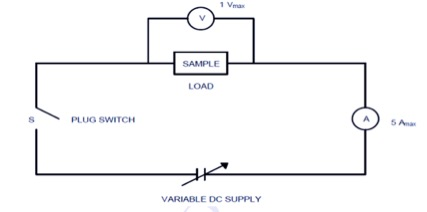
\includegraphics[width = \linewidth]{figure_3_3}
                    \caption{\label{figure_3_3}Electrical properties test circuitry}
                \end{figure}

                \begin{align}
                    {Resistance,}\quad & {R} = \frac{V}{I} \label{eq:equation_3}\\
                    {Resistivity,}\quad& {\rho} = \frac{{R} * {A}}{l}\label{eq:equation_4}\\
                    {Conductivity,}\quad & {G} = \frac{1}{\rho}\label{eq:equation_5}
                \end{align}
                \text{where}\\
                ${V =}$ Voltage in $\rm{V}$ (Volts)\\
                ${I =}$ Current in $\rm{A}$ (Ampere)\\
                ${R =}$ Resistance in $\rm{\Omega}$(Ohms)\\
                ${\rho =}$ Resistivity in $\rm{\Omega}$-m (Ohm-meter)\\
                ${G =}$ conductivity in $\rm{S}$/m (Siemen per meter)\\
                ${A =}$ Area in m$^2$ (square-meter)

        \section{\raggedright Result and Analysis}
            \subsection{\raggedright X-ray Diffraction Analysis}
                The diffractogram pattern was generated using a Cu-K$\alpha$ powder X-ray Diffractometer, Rigaku D/Max-111C, with Braggs 2$\theta$ scale from 10\degree to 45\degree. \ref{fig:figure_4_1} illustrates the XRD pattern of AA6061 + 0 wt.\% Chitosan. The diffractogram of unreinforced alloy reveals peaks of major \ch{Ca2Al3SIO4}, \ch{CaCO3}, \ch{Ca2SIO4}, and \ch{Ca(OH)2}, indicating a contaminated alloy with elevated elemental presence of Ca. AA6061 + 3wt.\%. 3 wt.\% Chitosan reinforced sample generates an XRD pattern with observed peaks with that of the unreinforced alloy nevertheless the pattern includes hydroxyapatite, \ch{Ca10(PO4)6(OH)2}. Result patterns \ref{fig:figure_4_3}, \ref{fig:figure_4_4} and \ref{fig:figure_4_5} is suggestive of presence of the \ch{Ca10(PO4)6(OH)2} biogenic compound in developed composite with 6, 9 and 12 wt.\% Chitosan respectively. The patterns are observed to increasing hydroxyapatite phases intensities with rising weight proportions of agro-waste, chitosan. The numerous occurrences of hydroxyapatite, \ch{Ca2Al3SIO4} and other phases in the XRD data substantiates evidence of organic matter convoluted in alloy matrix during composite coalescence.
                \begin{figure}[H]
                    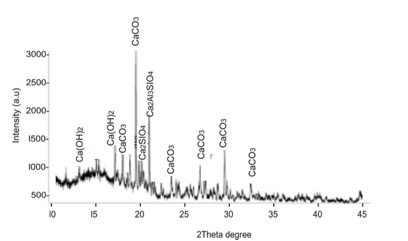
\includegraphics[width = \linewidth]{figure_4_1}
                    \caption{\label{fig:figure_4_1} XRD pattern of as-cast AA6061}
                \end{figure}
                \begin{figure}[H]
                    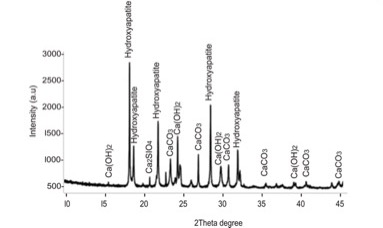
\includegraphics[width = \linewidth]{figure_4_2}
                    \caption{\label{fig:figure_4_2} XRD pattern of AA6061 + 3wt.\% chitosan}
                \end{figure}
                \begin{figure}[H]
                    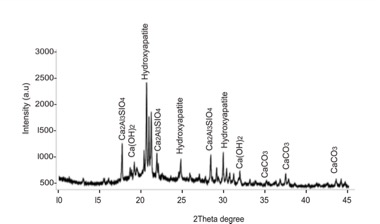
\includegraphics[width = \linewidth]{figure_4_3}
                    \caption{\label{fig:figure_4_3}  XRD pattern of AA6061 + 6 wt.\% chitosan}
                \end{figure}
                \begin{figure}[H]
                    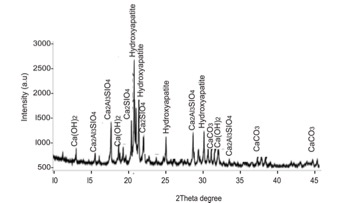
\includegraphics[width = \linewidth]{figure_4_4}
                    \caption{\label{fig:figure_4_4} XRD pattern of 9 wt.\% chitosan}
                \end{figure}
                \begin{figure}[H]
                    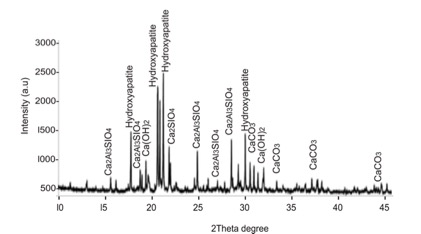
\includegraphics[width = \linewidth]{figure_4_5}
                    \caption{\label{fig:figure_4_5} XRD pattern of 12 wt.\% chitosan}
                \end{figure}
            \subsection{\raggedright Mechanical Properties}
                Mechanical characterization of chitosan reinforced composites performed using SM1000 tensile tester is demonstrated in figure 4.6, and 4.7 respectively. The maximum percentage elongation at ultimate tensile strength (UTS) was 2.334 \% for the unreinforced alloy, which declined with addition of chitosan reinforcement. 
                %Figure 4.6 
                depict reduced strain at UTS as weight proportion of chitosan reinforcements increased in the alloy matrix. Nevertheless, tensile strength enhanced sporadically with higher weight proportions of chitosan reinforcement. Hence, 12wt. \% chitosan possessed highest ultimate tensile strength of 114.92 MPa; a 38.4 \% increase in the mechanical property as seen in \ref{fig:figure_4_7}. Similarly, evaluations carried out using a Brinell’s hardness tester indicate sporadic improvements in hardness are illustrated in figure 4.8. The highest harness 60.2 HRB observed in 9 wt. \% chitosan reinforced sample indicated 4.88 \% improvement over as-cast AA6061 hardness (57.4 HRB), however, hardness perceptibly declined as more chitosan reinforcement. Yet, 3 wt.\% and 6 wt.\% chitosan reinforced AA6061 developed higher resistance to local deformation, 59.2 HRB and 57.8 HRB, than the unreinforced alloy. Results show insufficient improvement in aluminium matrix composite reinforced with 6 wt.\% chitosan over that of 3 wt.\% chitosan.
                \begin{figure}[H]
                    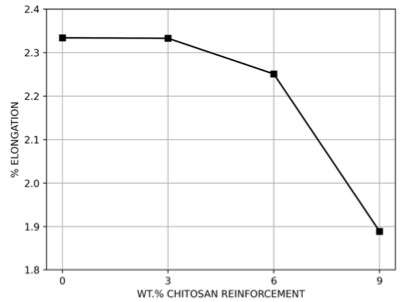
\includegraphics[width = \linewidth]{figure_4_6}
                    \caption{\label{fig:figure_4_6} \% elongation of aluminium matrix composites}
                \end{figure}
                \begin{figure}[H]
                    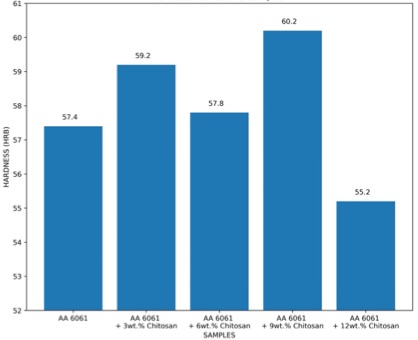
\includegraphics[width = \linewidth]{figure_4_7}
                    \caption{\label{fig:figure_4_7} Hardness of aluminium matrix composites}
                \end{figure}
                \begin{figure}[H]
                    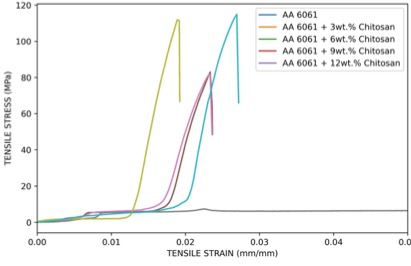
\includegraphics[width = \linewidth]{figure_4_8}
                    \caption{\label{fig:figure_4_8} Tensile Strength of aluminium matrix composite}
                \end{figure}
            \subsection{\raggedright Electrical and Thermal Conductivity}
                Electrical conductivity aluminium varies considerably between 30 $\rm{S}$/m and 65 $\rm{S}$/m, depending upon the metal's chemical composition and physical properties \citep{TheAluminiumAssociation2015,Wang2021}. \ref{fig:figure_4_9} show non-linear trend in electrical conductivity for the synthesized aluminium matrix composites. The evaluated electrical conductivity is maximum at 38.20 $\rm{S}$/m for 12wt.\% reinforced aluminium composite, while conductivity decrease is observed in 0, 3, 6, 9 wt.\% samples with values 37.81, 36.21, 36.61, 35.49 $\rm{S}$/m. A marginal rise occurred in 6 wt.\% chitosan reinforced sample, however, it represented no improvements to the conductivity of unreinforced alloy. An analogously inverse trend is established in \ref{fig:figure_4_10} where electrical resistivity peaks at 0.028 $\omega$m in 9 wt.\% chitosan reinforced sample followed by a decrease for the 12 wt.\% chitosan sample, 0.026 $\omega$m. Thus, further research should be carried out on aluminium alloy, AA 6061, reinforced with chitosan of weight proportions above 12\% to attain substantial improvements in electrical conductivity.
                \begin{figure}[H]
                    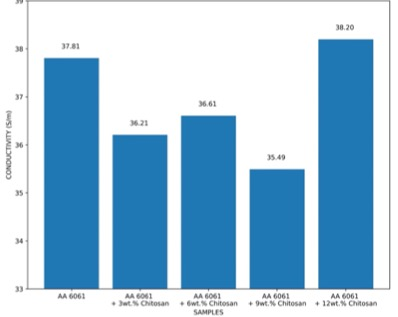
\includegraphics[width = \linewidth]{figure_4_9}
                    \caption{\label{fig:figure_4_9} Conductivity of aluminium matrix composites}
                \end{figure}
                \begin{figure}[H]
                    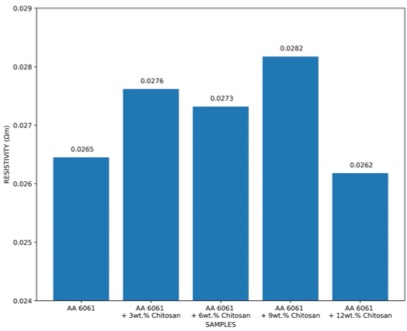
\includegraphics[width = \linewidth]{figure_4_10}
                    \caption{\label{fig:figure_4_10} Resistivity of aluminium matrix composites}
                \end{figure}

                The heat transfer coefficient is an important thermal property in the selection of materials for industrial use. In \ref{fig:figure_4_11}, the conductive heat transfer coefficient is represented for unreinforced alloy and each of the developed composites. The calculated mean heat transfer coefficient for the composites reinforced with 3, 6, 9 and 12 wt.\% chitosan increased with the increasing weigh proportions from 124.16 to 189.40 W/m$\degree$C, as seen in \ref{table:table_4_1}. However, the addition of chitosan failed to improve the overall thermal conductivity of the unreinforced alloy AA6061, which was obtained as 362.97 W/m$\degree$C. Thus, while the reinforcement reduced the thermal contact resistance between grains in the alloy matrix, its composition of silicon, calcium, and oxygen which are majorly poor thermal conductor with low thermal conductivity resulted in an overall thermal conductivity decrease.

                Similarly, results obtained from the addition of graphite-silicon carbide to aluminium alloy show lower thermal conductivity with added hybrid reinforcement of high silicon content compared to that of the as-cast alloy \citep{Krishna2016Microstructural}. Therefore, the reinforcement resulted in increased density of alloy matrix structure, limiting the flow of electrons. The results obtain still show high thermal conductivity for the AA6061- chitosan composite, which is suitable for electronic packaging requiring heat management such as fins for microprocessor units in computers.
                \begin{figure}[H]
                    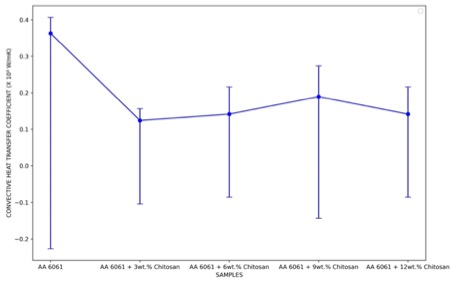
\includegraphics[width = \linewidth]{figure_4_11}
                    \caption{\label{fig:figure_4_11} Graph of Heat transfer coefficient of aluminium matrix composites}
                \end{figure}

                \begin{table}[H]
                    \caption{\label{table:table_4_1} Heat transfer coefficient of aluminium matrix composites\\} 
                    \begin{tabular*}{0.5\textwidth}{x{0.5 \linewidth} x{0.4\linewidth}}
                        \hline
                        Sample & Conductive Heat Transfer Coefficient (W/mK) \\ [0.5ex]  % refers to spacing between header row and nex row.
                        \hline
                        AA 6061 &   362.97\\[1em]
                        AA 6061 + 3 wt.\% Chitosan  &   141.59\\
                        AA 6061 + 6 wt.\% Chitosan  &   189.40\\
                        AA 6061 + 9 wt.\% Chitosan  &    141.59\\
                        AA 6061 + 12 wt.\% Chitosan &   124.16\\
                        [1ex]
                        \hline
                    \end{tabular*}
                \end{table}
            \subsection{\raggedright SEM/EDS analysis}
                Morphological characterization of aluminium was obtained using Scanning Electron Microscopy (SEM) and Energy Dispersive Spectroscopy (EDS) techniques. Figure 4.12 a and b shows microscopic and compositional data on the unreinforced AA6061, aluminium alloy, sample obtained through SEM and EDS respectively.
                
                As observed in figure 4.13, 0.2 $\mu$m sized fibrous particulates of the 3 wt.\% chitosan reinforcements surround the darker well-defined alloy matrix seen in figure 4.12. Minimal voids approximately 10 $\mu$m are observed in the composite structure. Compositionally, the EDS result of the composite showed increased calcium and oxygen contents of the composite indicating intrinsic. In contrast, this indicates stirred both of which are found abundantly in the chitosan reinforcement.

                From figure 4.14, near perfect dispersion of chitosan forming link structure that occupy most of the grain boundary. The serve to distribute a for the telling to the improved tensile performance of the composite. EDS analysis show distinguishable growth in the percentage of calcium and oxygen elements in the composite. A result of more chitosan constituents to convolute with intermetallic phases of the alloy matrix.

                The 9 wt.\% chitosan reinforced composite morphology observed in figure 4.15 show meticulously arranged composite structure previously observed in figure 4.13 and 4.14. However, more chitosan particulate innocuously occupies grain boundary voids in even distribution as observed in figure 4.15 resulting in a higher load bearing capacity. Thus, a further improved mechanical performance is observed from the composite mechanical characterization. EDS data show rising oxygen content partly responsible for its electrical resistance with pronounced Silicon, Iron, Carbon and Magnesium constituents.

                SEM images illustrated in figure 4.16, show slight agglomeration of produced during composite synthesis of the 12 wt.\% chitosan and aluminium alloy. Reinforcements appear to be laid along boundary voids of alloy structure to connect adjacent grains of the continuous matrix. The EDS analysis identifies prominent calcium and oxygen peaks and highlights the rising elemental carbon composition indicating rich biogenic material presence within the composite.
                \begin{figure}[H]
                    \begin{subfigure}{.25\textwidth}
                        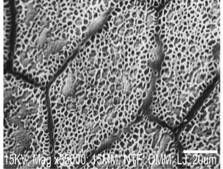
\includegraphics[width=\linewidth]{figure_4_12_a}
                        \label{fig:figure_4_12_a}
                    \end{subfigure}%
                    \begin{subfigure}{.25\textwidth}
                        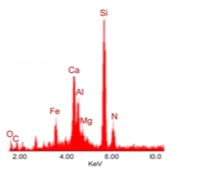
\includegraphics[width=\linewidth]{figure_4_12_b}
                        \label{fig:figure_4_12_b}
                    \end{subfigure}
                    \caption{SEM image of unreinforced AA6061 sample (b) EDS of sample}
                \end{figure}

                \begin{figure}[H]
                    \begin{subfigure}{.25\textwidth}
                        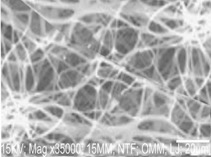
\includegraphics[width=\linewidth]{figure_4_13_a}
                        \label{fig:figure_4_13_a}
                    \end{subfigure}%
                    \begin{subfigure}{.25\textwidth}
                        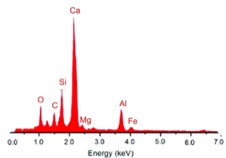
\includegraphics[width=\linewidth]{figure_4_13_b}
                        \label{fig:figure_4_13_b}
                    \end{subfigure}
                    \caption{SEM image of 3 wt.\% chitosan reinforced AA6061 sample (b) EDS of sample}
                \end{figure}
                \begin{figure}[H]
                    \begin{subfigure}{.25\textwidth}
                        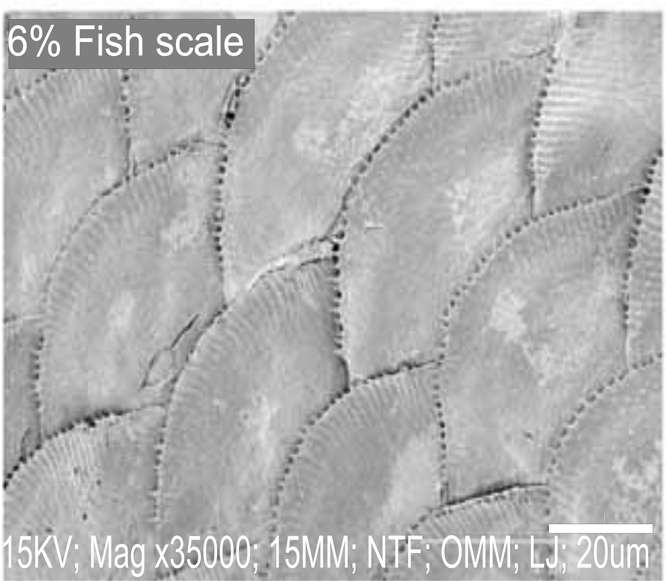
\includegraphics[width=\linewidth]{figure_4_14_a}
                        \label{fig:figure_4_14_a}
                    \end{subfigure}%
                    \begin{subfigure}{.25\textwidth}
                        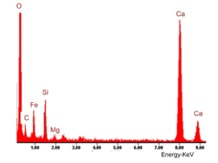
\includegraphics[width=\linewidth]{figure_4_14_b}
                        \label{fig:figure_4_14_b}
                    \end{subfigure}
                    \caption{SEM image of 6 wt.\% chitosan reinforced AA6061 sample (b) EDS of sample}
                \end{figure}

                \begin{figure}[H]
                    \begin{subfigure}{.25\textwidth}
                        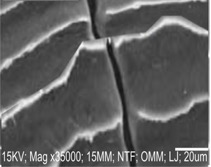
\includegraphics[width=\linewidth]{figure_4_15_a}
                        \label{fig:figure_4_15_a}
                    \end{subfigure}%
                    \begin{subfigure}{.25\textwidth}
                        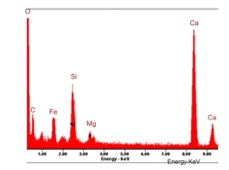
\includegraphics[width=\linewidth]{figure_4_15_b}
                        \label{fig:figure_4_15_b}
                    \end{subfigure}
                    \caption{SEM image of 9 wt.\% chitosan reinforced AA6061 sample (b) EDS of sample}
                \end{figure}

                \begin{figure}[H]
                    \begin{subfigure}{.25\textwidth}
                        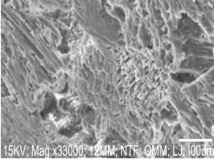
\includegraphics[width=\linewidth]{figure_4_16_a}
                        \label{fig:figure_4_16_a}
                    \end{subfigure}%
                    \begin{subfigure}{.25\textwidth}
                        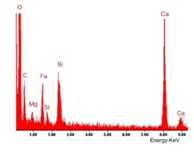
\includegraphics[width=\linewidth]{figure_4_16_b}
                        \label{fig:figure_4_16_b}
                    \end{subfigure}
                    \caption{SEM image of 12 wt.\% chitosan reinforced AA6061 sample (b) EDS of sample}
                \end{figure}

        \section*{\raggedright Conclusions}
            Chitosan of 90 microns sieve-size was successfully coalesced in aluminium alloy, AA 6061, matrix via stir casting in weight proportion 3 \%, 6 \%, 9 \% and 12 \%. The characterization of the developed composites resulted in the following conclusions:
            \begin{itemize}
                \item 
                    Hardness of the developed composites improved with higher concentration of chitosan particulate; 9 wt.\% chitosan reinforced sample developed a substantial 4.88 \% improvement.
                
                \item 
                    Composite coalesced with Particulate Reinforcement high percentage of contained carbon and oxygen, and as well as biogenic phase hydroxyapatite.

                \item 
                    Reinforcement particles were evenly dispersed in alloy matrix with slight agglomeration observed in the 12 wt.\% chitosan reinforced sample.

                \item 
                    The electrical conductivity of aluminium matrix composite reinforced with chitosan reduced compared to unreinforced AA6061 because of introduction of insulation from chitosan reinforcement.
                
                \item     
                    The synthesized composites showed enhanced tensile strength performance with a 25.8 \% increase observed the 12 wt.\% chitosan reinforced sample.
                \item 
                    Stir casted AA6061/chitosan provided reduced conductive heat transfer coefficient compared to as-cast AA 6061.
            \end{itemize}

        \section*{\raggedright Declaration of Competing Interest}
            The authors declare that they have no known competing financial interests or personal relationships that could have appeared to influence the work reported in this paper.

        \section*{Appreciation}
            This work is based on research conducted at the mechanical engineering department in Covenant University, Ota, Ogun State, Nigeria.

        \bibliographystyle{apalike}
        \bibliography{ref-extracts}

    \end{multicols}



    
\end{document}